% This file was converted to LaTeX by Writer2LaTeX ver. 1.0.2
% see http://writer2latex.sourceforge.net for more info
\documentclass[12pt]{article}
\usepackage[left=1.50cm, right=1.00cm, top=2.00cm, bottom=2.00cm]{geometry}
\usepackage[ascii]{inputenc}
\usepackage[T1]{fontenc}
\usepackage[english]{babel}
\usepackage{amsmath}
\usepackage{amssymb,amsfonts,textcomp}
\usepackage{array}
\usepackage{hhline}
\usepackage{graphicx}
\usepackage{setspace}
\def\rosario{9}
\def\novena{4}
\title{Doa Rosario Roh Kudus Hari ke \rosario{} dan Novena Roh Kudus Hari ke \novena{}}
\author{Lingkungan St. Theresia}
\date{2016-05-09}
\def\petugasA{\textbf{Riani}}
\def\petugasB{\textbf{Lintang}}
\begin{document}
	
 \maketitle
\onehalfspacing
petugasA: Ibu, Bapak dan teman-teman , marilah kita awali doa kita pada
malam hari ini dengan Lagu Pembuka, yang akan dipimpin oleh Mas Ari

\section{Lagu: Dengar Dia Panggil
Nama Saya }
\begin{quote}
\textit{
Dengar dia panggil nama saya\\
Dengar dia panggil nama mu\\ 
Dengar dia panggil nama saya\\
Juga dia panggil nama mu\\ 
Oh girang lah aleluya,  \\
oh giranglah puji Tuhan\\ 
Yesus amat cinta pada saya\\ 
oh giranglah\\  
Kujawab ya ya ya \\
kujawab ya ya ya \\
Kujawab ya Tuhan \\
kujawab ya Tuhan \\ 
Kujawab ya ya ya
}
\end{quote}

\petugasA: 

P. Demi nama Bapa, dan Putera, dan Roh Kudus.

U. Amin.

P. Semoga Allah Bapa serta Putera-Nya, Tuhan kita Yesus Kristus,
memberikan Roh Kudus kepada kita.

U. Sekarang dan selama-lamanya.

Ibu, Bapak dan teman-teman yang terkasih dalam Kristus, Selamat malam,
Berkah Dalem..

Malam ini merupakan malam ke 9 kita semua dengan setia mendaraskan doa
Rosario, serta Doa Novena hari ke 4. Dan kita bersyukur karena masih
diperkenankan bersama-sama bergembira, berdoa dan memuliakan Yesus
melalui perantaraan Bunda Maria. 

Pada malam hari ini, kami kanak-kanak Yesus, akan bersama-sama memandu
doa Rosario serta doa Novena. Peristiwa Gembira akan kita ganti dengan
merenungkan Misteri Roh Kudus.  

\petugasA: 

Teman-teman dan Bapak ibu terkasih. Setelah Tuhan Yesus naik ke surga,
ibu Maria dan para rasul berkumpul di ruang makan lantai dua sebuah
rumah, bersama-sama berdoa MOHON TURUNNYA ROH KUDUS 

Marilah kita bersama ibu Maria dan para rasul berdoa dengan intensi
agar: 

Kita masing-masing beserta keluarga diberkati Tuhan dan dicurahi Roh
Kudus. 

Agar kuasa kegelapan diusir dari kita, keluarga dan rumah kita. 

Agar kita dianugerahi iman-pengharapan-kasih,
kebijaksanaan-kesucian-kesetiaan, kebahagiaan dan keceriaan, baik dalam
untung maupun malang. 

Agar kita diberi Kesehatan badan-jiwa, dan dibebaskan dari bahaya
jasmani-rohani. Pekerjaan yang lancar dan rejeki yang cukup. 

Agar kita kanak-kanak Yesus nantinya menjadi {\textquotedblleft}Pria
Utama{\textquotedblright} dan {\textquotedblleft}Wanita
Utama{\textquotedblright}. 

Lagu : Datanglah Roh Maha Kudus : MB : 448

Riani : Marilah berdoa. 

* Ya Allah / Engkau yang mengajar hati umat-Mu dengan penerangan Roh
Kudus. / Berilah kami, dengan pengantaraan Roh Kudus, KEBIJAKSANAAN
YANG SEJATI, / serta karunia SELALU MERASA GEMBIRA karena
penghiburan-Nya. / Demi Kristus, Tuhan dan pengantara kami.. Amin.

Fira : BACAAN KITAB SUCI : (Yesaya 11:2{}-3).

Ada seorang lumpuh berbaring di tepi kolam Betesda. Sudah 38 tahun dia
mau mengambil kesempatan pertama untuk mencelupkan tangannya ke kolam
ketika air kolam digoyangkan malaikat, supaya disembuhkan. Tapi tak
pernah berhasil, karena lumpuh. Tuhan Yesus datang padanya dan bertanya
{\textquotedblleft}Maukah engkau sembuh?{\textquotedblright}. Jawabnya
\emph{{\textquotedblleft}Ya Tuhan saya mau{\textquotedblright}}. Lalu
\emph{Tuhan Yesus ber-sabda kepadanya {\textquotedblleft}Bangunlah dan
angkatlah tilammu dan berjalanlah}{\textquotedblright} Maka orang itu
sembuh.

Demikianlah Sabda Tuhan

Inti dari bacaan tersebut adalah :

 1) Orang lumpuh tersebut gambaran kita dan umat manusia yang berdosa
(Tak mampu berdoa dan beramal. Doa dan amal pendosa itu palsu). 

2) Kedatangan Tuhan Yesus ke dunia adalah untuk memulihkan Roh Kudus dan
kekuatan illahi dalam umat manusia. Menjadi kuat, baik, dan suci.

Fira : Marilah kita doakan DOA MOHON TUJUH KARUNIA ROH KUDUS. 

Bersama : Datanglah, ROH NASIHAT. Dampingilah kami dalam hidup yang
penuh gejolak ini. Tunjukkanlah kepada kami:  yang baik dan benar;
Tuhan serta rahmat-Nya. Dan doronglah kami mencintai-Nya dan menjauhi
dosa. 

Putri : Datanglah, ROH PENGERTIAN. Terangilah budi kami agar dapat
melihat dan memilah-milah baik-buruk benar-salah. Memahami ajaran
Yesus, serta melihat hasilnya yang baik kalau kami melaksanakannya. 

Putra : Datanglah, ROH YANG MENGENAL ALLAH. Ajarilah kami agar mampu
{\textquotedblleft}melihat{\textquotedblright} Tuhan dan rahmat-Nya di
sekitar kami. {\textquotedblleft}Melihat{\textquotedblright}
ke-selamatan dalam tugas yang berat.
{\textquotedblleft}Melihat{\textquotedblright} sifat-sementara dari hal
yang duniawi. Dan {\textquotedblleft}melihat{\textquotedblright} yang
jahat serta malapetaka yang diakibatkannya. 

Putri : Datanglah, ROH TAKUT KEPADA ALLAH. Ajarlah kami takut kepada
Tuhan. Dan membenci dosa serta takut kepada akibat buruk dari padanya.

Putra : Datanglah, ROH HIKMAT KEBIJAKSANAAN. Ajarilah kami menjadi
bijaksana. Mampu menghargai, memilih, dan mencintai yang baik, terutama
cita-cita surga, walaupun berat dan pahit. Agar kami lebih mencintai
Tuhan dan kesucian, daripada diri kami sendiri. Dan agar kami membenci
yang jahat dan dosa, serta Kau bebaskan daripadanya 

Putri : Datanglah, ROH KESALEHAN. Dampingilah dan bimbinglah kami untuk
melaksanakan yang baik dan yang berkenan pada-Mu. Menjadi orang yang
tahu berterima kasih atas segala kebaikan Tuhan. Agar kami taat dan
mengabdi Tuhan di manapun kami berada. Menunaikan tugas sebagai anggota
keluarga dan masyarakat. Menjadi teladan-kesalehan bagi lingkungan
kami. Serta mampu menggunakan hal-hal duniawi dengan bijaksana, hanya
demi kemuliaan-Mu saja. 

Bersama : Datanglah, ROH KEPERKASAAN. Kuatkanlah hamba-Mu yang lemah
ini, agar setia melaksanakan kebaikan dan kebenaran dalam hidup kami
sehari-hari, serta menjauhi yang jahat, betapapun berat dan pahitnya.
Agar kami tabah dalam segala kesulitan dan derita. Kuatkanlah kami
bilamana kami selalu memegang tangan-Mu yang senantiasa menuntun kami.
Amin. 

Fira : Marilah kita lanjutkan dengan BKL hari ke 9, yang akan dipimpin
oleh Bpk Neo.

Bp Neo

BKL HARI KE 9 : 

DOA ROSARIO ROH KUDUS

  [Warning: Image ignored] % Unhandled or unsupported graphics:
%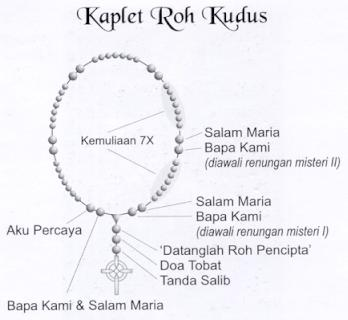
\includegraphics[width=12.672cm,height=11.665cm]{rosariorohkudus9-img1.jpg}
 

\petugasA:

Bapak Ibu yang terkasih dalam Kristus, kita akan mendoakan DOA ROSARIO
ROH KUDUS. Namun karena kita semua tidak membawa Rosario Roh Kudus
seperti pada gambar, maka kita tetap memakai Rosario biasa, namun
dengan urutan seperti ROSARIO ROH KUDUS, dan kemuliaan yang seharusnya
7x kita ganti 10x, sesuai jumlah manik pada Rosario biasa.

Kita awali dengan lagu Maria, MB : 542

\petugasB:

Tanda Salib : Demi nama Bapa, dan Putera, dan Roh Kudus.

Doa Tobat : Saya mengaku, kepada ....

Marilah kita doakan secara bergantian  doa  DATANGLAH, YA ROH PENCIPTA
(Puji Syukur, No. 565).

Bersama : Datanglah, ya Roh Pencipta. Hati kami kunjungilah. Penuhi
dengan RahmatMu. Jiwa kami ciptaanMu. 

Putri : Kau digelari Penghibur, karunia Allah yang luhur. Kau hidup,
api, dan kasih, dan pengurapan ilahi. 

Putra : Dikau sapta karunia, dan tangan kanan ilahi. Engkau yang Bapa
janjikan Kau pergandakan bahasa.

Putri : Sinari hati umatMu, dan curahkanlah cintaMu. Semoga Dikau
kuatkan yang rapuh dalam tubuhnya.

Putra : Halaulah musuh umatMu. Berilah kami damaiMu, agar dengan
tuntunanMu kami hindarkan yang jahat. 

Putri : Buatlah kami mengenal serta mengimani terus Bapa dan Putra yang
tunggal dan Engkau Roh keduanya. 

Bersama : Dipujilah Allah Bapa dan Putra yang sudah bangkit, serta Roh
Kudus Penghibur, kini dan sepanjang masa. Amin. 

\petugasA:

Misteri Pertama: {\textquotedbl}Dari Roh Kuduslah Yesus dikandung
Perawan Maria.{\textquotedbl} Renungan  {\textquotedblleft}Roh Kudus
akan turun atasmu dan kuasa Allah yang Mahatinggi akan menaungi engkau;
sebab itu anak yang akan kau lahirkan itu akan disebut kudus, Anak
Allah.{\textquotedblright}

\petugasB: Dengan tekun, mintalah bantuan dari Roh Ilahi serta perantaraan
Bunda Maria untuk mengikuti kebajikan-kebajikan Yesus Kristus,
contohlah segala kebajikan-Nya, sehingga kita dapat menjadi serupa
dengan citra Putra Allah.

 Bapa Kami {\dots}(1x) Salam Maria {\dots} (1x) Kemuliaan ... (10x)

\petugasA:

Misteri Kedua:{\textquotedbl}Roh Allah turun atas Yesus.{\textquotedbl}
Renungan : {\textquotedblleft}Sesudah dibaptis, Yesus segera keluar
dari air, dan pada waktu itu juga langit terbuka dan Ia melihat Roh
Allah seperti burung merpati turun ke atasnya.{\textquotedblright}

\petugasB:

Peliharalah dengan penuh kesungguhan anugrah yang tak ternilai, rahmat
pengudusan yang dicurahkan dan ditanamkan dalam jiwa kita oleh Roh
Kudus pada saat pembabtisan. Peganglah dengan teguh janji baptis yang
telah kita ucapkan: tingkatkan iman, harapan dan cinta kasih melalui
tindakan nyata, serta hiduplah sebagai anak-anak Allah dan anggota
Gereja Allah yang sejati agar kelak kita dapat memperoleh warisan
surgawi.

 Bapa Kami {\dots}(1x) Salam Maria {\dots} (1x) Kemuliaan ... (10x)

\petugasA:

Misteri Ketiga:{\textquotedbl}Oleh Roh Kudus, Yesus dibimbing menuju
padang gurun untuk dicobai.{\textquotedbl} Renungan :
{\textquotedblleft}Yesus, yang penuh dengan Roh Kudus, kembali dari
Sungai Yordan, lalu dibawa oleh Roh Kudus ke padang gurun. Di situ Ia
tinggal empat puluh hari lamanya dan dicobai Iblis.{\textquotedblright}

\petugasB: Bersyukurlah selalu atas ketujuh karunia Roh Kudus yang dicurahkan
pada kita saat menerima Sakramen Penguatan: Roh kebijaksanaan,
pengertian, nasihat, keperkasaan, pengenalan akan Allah, kesalehan, dan
rasa takut akan Allah. Serahkan diri kita dengan setia kepada bimbingan
Ilahi-Nya, sehingga di atas segala godaan dan pencobaan hidup kita
berlaku secara perkasa sebagai seorang Kristen sejati dan prajurit
Kristus yang berani.

Bapa Kami {\dots}(1x) Salam Maria {\dots} (1x) Kemuliaan ... (10x)

\petugasA:

Misteri Keempat:{\textquotedbl}Peranan Roh Kudus dalam
Gereja.{\textquotedbl} Renungan : {\textquotedblleft}Tiba-tiba turunlah
dari langit suatu bunyi seperti tiupan angin keras yang memenuhi
seluruh rumah di mana mereka duduk.... Maka penuhlah mereka dengan Roh
Kudus, lalu mereka mulai berkata-kata ... tentang perbuatan-perbuatan
besar yang dilakukan Allah.{\textquotedblright}

\petugasB: Bersyukurlah kepada Tuhan karena Ia menjadikan kita sebagai
anggota Gereja-Nya yang selalu dijiwai dan diarahkan oleh Roh Kudus,
Roh yang diturunkan ke dunia untuk tugas itu pada hari Pentekosta.
Dengarlah dan patuhilah Takhta Suci, wakil Roh Kudus yang tidak dapat
salah, serta Gereja, pilar dan dasar kebenaran. Junjunglah
ajaran-ajarannya dan belalah hak-haknya.

 Bapa Kami {\dots}(1x) Salam Maria {\dots} (1x) Kemuliaan ... (10x)

\petugasA:

Misteri Kelima:{\textquotedbl}Roh Kudus dalam jiwa-jiwa orang
beriman.{\textquotedbl} Renungan : {\textquotedblleft}Tidak tahukah
kamu, bahwa tubuhmu adalah bait Roh Kudus yang diam di dalam
kamu?{\textquotedblright}; {\textquotedblleft}Janganlah padamkan
Roh.{\textquotedblright}; {\textquotedblleft}Dan janganlah kamu
mendukakan Roh Kudus Allah, yang telah memateraikan kamu menjelang hari
penyelamatan.{\textquotedblright}

\petugasB: Sadarilah keberadaan Roh Kudus dalam diri kita, peliharalah dengan
seksama kemurnian tubuh dan jiwa, ikutilah dengan setia bimbingan
Ilahi-Nya, sehingga kita dapat menghasilkan buah-buah Roh: kasih,
sukacita, damai sejahtera, kesabaran, kemurahan hati, kebaikan,
kesetiaan, kelemah lembutan, iman, kerendahan hati, penguasaan diri,
dan kemurnian.

 Bapa Kami {\dots}(1x) Salam Maria {\dots} (1x) Kemuliaan ... (10x)

Aku Percaya ... Bapa Kami ... Salam Maria ...

Riani 

PENUTUP.

P. Semoga Tuhan beserta kita.

U. Sekarang dan selama-lamanya.

P. Semoga kita semua, beserta keluarga dan karya kita, diberkati oleh
Allah yang mahakuasa : + Bapa, dan Putera, dan Roh Kudus.

U. Amin.

P. Bapak ibu dengan ini Novena Roh Kudus, hari ke- 3 sudah selesai.

U. Syukur kepada Allah.

 Lagu Penutup:  CURAHKAN RAHMAT DALAM HATIKU.

Refr. Curahkan rahmat dalam hatiku. Ciptakan hati, dan semangat baru.

{}-1- Engkau Kucucikan dan Kubersihkan dari cinta-diri. Engkau
Kuhidupkan. Dan Kukobarkan cinta di hati. Refr. 

{}-2- Hatimu yang kaku, keras, dan beku, Kuambil darimu. Ambillah
dari-Ku semangat baru dalam karyamu. Refr.

\end{document}
